
\subsection{Lecture de tension des modules}
	\paragraph*{}
	Nous désirons avoir une lecture de tension très précise sur toute la plage d'utilisation des modules. Le circuit doit consommer un minimum de courant, être robuste, modulable et précis. Le circuit doit aussi faciliter la vérification technique.
	
	\subsubsection*{Solution commercial}
	\paragraph*{}
	Il existe sur le marché plusieurs circuit qui s'occupe de lire la tension des modules et de communiquer l'information à un microcontrôleur. Les fonctionnalités et le nombre de modules supportés varient d'un vendeur à l'autre. Les points communs sont : 

	\begin{multicols}{2}
		\begin{itemize}
			\item[$\bullet$] Le circuit peut être alimenté par les modules;
			\item[$\bullet$] Consommation de courant de quelque mA lorsque le circuit prend les mesures et quelque $\mu$A lorsqu'il est en veille;
			\item[$\bullet$] Solution compacte;
			\item[$\bullet$] Lecture précise;
			\item[$\bullet$] Les modules doivent être branchés dans l'ordre;
			\item[$\bullet$] Économique;
			\item[$\bullet$] Fonctionnement bien documenté.
		\end{itemize}
	\end{multicols}

	\paragraph*{}
	Cette solution est réalisable et demande surtout de bien lire et comprendre la documentation. Le LTC6804 de Linear Technology a été retenu pour son nombre de modules maximum, son prix et sa simplicité d'implémentation. Cette solution répond à la majorité des spécifications mais elle n'apporte cependant rien de nouveau au système présentement utilisé et elle ne facilite pas la vérification technique. 
	
	\newpage
	
	\subsubsection*{Isolation des lectures}
	\paragraph*{}
	La vérification technique sera beaucoup plus facile si les différentes lectures de tensions sont isolées. Ce point est décrit dans la section Facilité les manipulations lors des vérifications techniques. 
	
	\paragraph*{}
	L'isolation amène plusieurs avantages :
	
	\begin{itemize}
		\item[$\bullet$] Les modules n'ont plus besoin d'être branchés en ordre, ce qui élimine ce risque d'erreur humaine;
		\item[$\bullet$] Il est possible de débrancher une seule cellule pour venir ensuite la remplacer par une alimentation variable;
		\item[$\bullet$] Le filage dans la batterie peut être mieux organisé et optimisé.
	\end{itemize}

	\paragraph*{}
	Cette solution comporte cependant plusieurs désavantage :
	
	\begin{itemize}
		\item[$\bullet$] Consomme plus de courant (quelque mA par module lors des lectures);
		\item[$\bullet$] Demande plus de composantes;
		\item[$\bullet$] Plus difficile à implémenter;
		\item[$\bullet$] Plus dispendieux.
	\end{itemize}
	
	\paragraph*{}
	Ces différents désavantages ne sont pas majeurs dans le contexte d'Éclipse, la consommation de courant reste insignifiante comparé à ce que le moteur et le reste des circuits consomment. Le nombre de composant peut être limité en utilisant la bonne topologie et le prix de la carte peut être plus élevé tant qu'il respecte le budget. 
	
	\subsubsection*{Circuit analogique}
	\paragraph*{}
	Une solution relativement simple et qui ne comporte pas beaucoup de composante est montré à la figure \ref{fig:HCNR201}. Ce circuit très compacte et simple n'est pas assez précis puisque le gain entre les deux photodiodes varie de 5\% pour le HCNR201. Cette erreur fait en sorte que le circuit ne répond pas aux spécifications de +/- 10mV.  
	
	\begin{figure}[H]
		\centering
		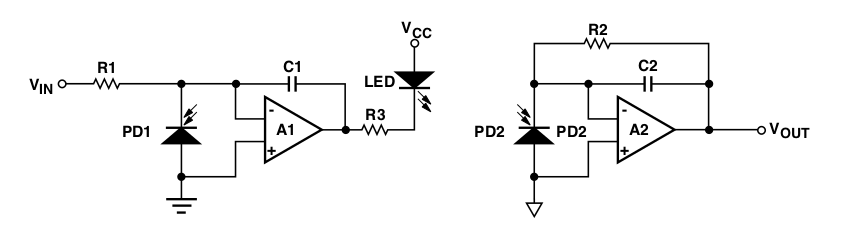
\includegraphics[scale = 0.5]{Images/Analogique.png}
		\caption{Circuit de lecture de tension isolé analogique \cite{HCNR201}}
		\label{fig:HCNR201}
	\end{figure}


	\newpage
	\subsubsection*{Lecture d'un voltage de référence avec un ADC}
	\paragraph*{}	
	Pour éliminé l'erreur causé par l'amplificateur et l'isolateur tout en réduisant au maximum le nombre de composants, l'ADC mesurerait un voltage de référence alors qu'il serait alimenté par le module comme présenté à la figure \ref{fig:adc_vref}. Puisque le voltage à l'entrée est connu, la tension du module est donné par l'équation \ref{eq:vref}.
	
	\begin{align}
		V_{Module} = \dfrac{V_{REF}}{Valeur~ADC} \cdot 2^{~nb~Bits~adc}
		\label{eq:vref}
	\end{align}
	
	\begin{figure}[H]
		\centering
		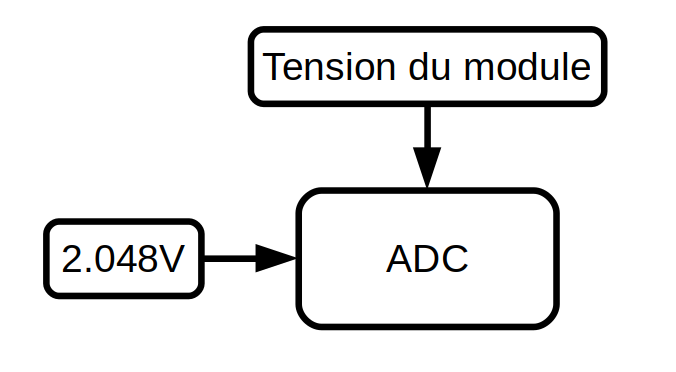
\includegraphics[scale=0.3]{Images/Voltage_reference.png}
		\caption{Lecture d'un voltage de référence avec un ADC}
		\label{fig:adc_vref}
	\end{figure}
	
	\paragraph*{}
	Le circuit mesure le LSB qui est donné par $V_{Module} / 2^{~nb~Bits~adc}$ pour  trouver la tension du module. Bien que cette technique fonctionne, les courbes de la tension du module et de la résolution ne sont pas linéaire par rapport au résultat du ADC. La valeur du voltage de référence à un impacte sur la courbe de la résolution. Plus il est bas, moins la courbe est linéaire et la résolution est moins bonne. Les figures \ref{fig:vmodule_vref} et \ref{fig:res_vref} montre les performances idéal du circuit à la figure \ref{fig:adc_vref} avec une référence de 2.048V et une plage de 2V à 4.2V pour la tension du module.
	
	\begin{figure}[H]
		\begin{minipage}{0.45\textwidth}
			\centering
			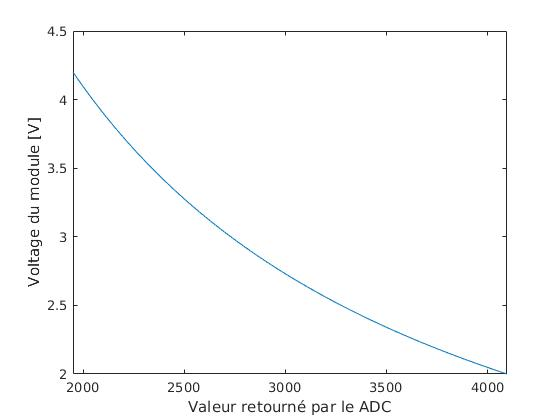
\includegraphics[scale=0.4]{Images/Vmodule_REF_2V.jpg}
			\caption{Tension du module en fonction des valeurs du ADC}
			\label{fig:vmodule_vref}
		\end{minipage}
		\hfill
		\begin{minipage}{0.45\textwidth}
			\centering
			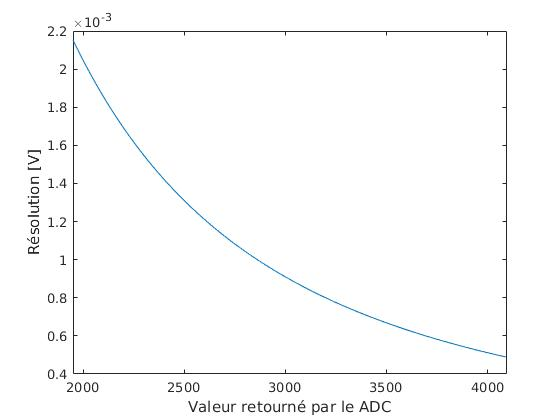
\includegraphics[scale=0.4]{Images/RES_REF_2V.jpg}
			\caption{Résolution en fonction des valeurs du ADC}
			\label{fig:res_vref}
		\end{minipage}	
	\end{figure}	
	
	\paragraph*{}
	L'écart maximal entre 2 bits est de 2.15 mA. Avec un ADC performant qui a une erreur de $\pm 1$ LSB, la lecture de tension à une erreur maximal de $\pm $ 2.15 mA lorsque le module est à 4.2V. Cette méthode correspond à la spécification qui demande d'être à $\pm $ 10 mA. L'ADC consomme et la tension de référence consomme très peu de courant, ils nécessitent très peu de composants externe et ils sont abordable. Afin d'avoir une très bonne précision, il est nécessaire de faire une calibration puisque la tolérance de la référence ($\pm$ 0.5 \%) est plus grande que celle de la spécification ($\pm 0.238 \% = \pm 10mV / 4.2V \cdot 100 \%$). Il existe des références avec des tolérances plus petite que $\pm 0.238$ mais elles sont beaucoup trop dispendieuse pour le projet puisqu'il faut en avoir une pour chaque module.    
	
	\paragraph*{}
	L'isolation de la mesure ce fait au niveau de la communication puisqu'il n'y a aucune erreur causé par l'isolateur de cette façon, contrairement à l'optocoupleur de la solution analogique. L'alimentation de l'isolateur et du ADC doivent dépasser la plage de lecture du module qui est de 2V à 4.5V.
	
	\paragraph*{}
	Cette solution est viable, elle respecte les spécifications et elle ne demande pas beaucoup de composantes. Le choix des circuits intégrés avec une alimentation qui va de moins de 2V à plus de 5V est toutefois très restreint. Le prix de l'isolateur et de l'ADC sont donc élevé et il est plus difficile de trouver un remplacement dans le cas ou un composant n'est plus manufacturé.   
	
	\subsubsection*{Configuration classique de l'ADC}
	\paragraph*{}
	
	
	
	
	
	
	
	
	
	
	
	
	
	
	
	
	
	
	
	
	
	
	